\documentclass{article}

\usepackage{graphicx}
\usepackage{subcaption}
\usepackage{amssymb}
\usepackage[utf8]{inputenc}
\usepackage[T1]{fontenc}

\renewcommand{\familydefault}{\sfdefault}
\usepackage[scaled=1]{helvet}
\usepackage[helvet]{sfmath}
\everymath={\sf}

\title{Reporte de Actividad 5}

\author{Diego Iván Moreno Campa}

\date{6 de Marzo, 2018}

\begin{document}

\maketitle

\bigskip

\section{Introducción}

Esta actividad es el quinto trabajo para la materia de Física computacional I en la licenciatura de Física.

El propósito de esta actividad es limpiar y organizar los datos para luego realizar un análisis utilizando Pandas en Python. A partir del archivo creado en la práctica anterior se creará un archivo que contenga únicamente columnas de datos de Fecha, CAPE y PW.

\section{Fundamentos}

En esta actividad se trabajara con conceptos como CAPE y PW, los cuales se explicaran a continuación:

\subsection{la energía potencial convectiva disponible (CAPE)}

la energía potencial convectiva disponible (o CAPE, por las siglas del inglés Convective Available Potential Energy) es un parámetro de estabilidad de uso difundido, que indica la cantidad de energía de empuje hidrostático disponible para una burbuja que acelera hacia arriba, el cálculo de dicho parámetro se muestra  en la figura 1. En este diagrama termodinámico, la región resaltada en naranja (positiva) entre el nivel de convección libre (NCL) y el nivel de equilibrio (NE) representa la CAPE.

\begin{figure}[ht!]
\centering
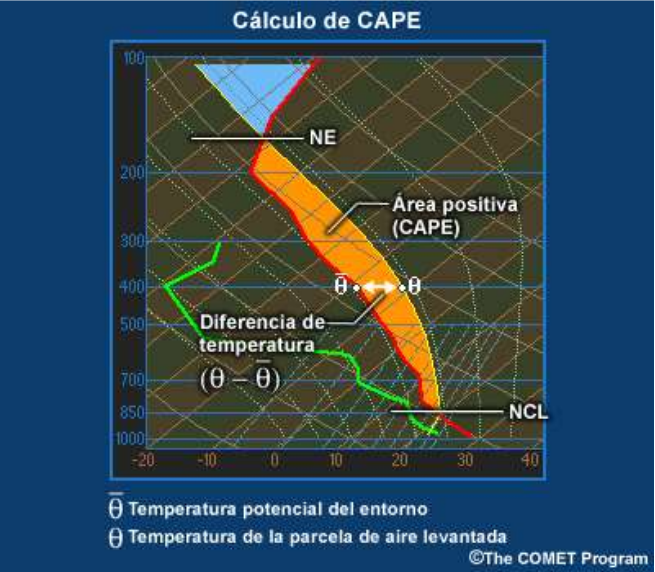
\includegraphics[width=0.6\linewidth]{cape.png}
\caption{Cálculo del CAPE. Fuente: Comet}
\end{figure}

Cuanto más alto sea el valor de CAPE, tanto mayor será el potencial de formación de tormentas fuertes e incluso severas. En el trópico, los valores típicos de CAPE son mucho más bajos que en las latitudes medias, excepto en los sistemas convectivos de mesoescala más intensos.

\subsection{Agua precipitable (PW)}

El agua precipitable es la cantidad total de vapor de agua atmosférico contenido en una columna vertical de unidad transversal de área que se extiende entre dos niveles específicos, comúnmente expresado en términos de altura a la que tal sustancia de agua se mantendría sí fuera completamente condensada y juntada en un recipiente de la misma unidad transversal.

\section{Procedimiento}

Primeramente se seleccionaron únicamente los datos que con los que se trabajaran en esta práctica, fecha, CAPE y PW, a partir del archivo \textit{sondeos.txt} creado en la práctica pasada, utilizando la siguiente instrucción: 
\begin{verbatim}
egrep -v 'PRES|hPa' sondeos.txt | egrep 'H2|CAPE|Precip' > df2017CAPE_PW.csv
\end{verbatim}

El archivo producido tiene texto repetido, por lo que se procede a limpiar el archivo obtenido en la práctica pasada utilizando comandos de EMACS para seleccionar y reemplazar el texto que se repetía por espacios o comas. Seleccionando el texto con el comando CTRL-(spacebar), las flechas y CTRL-w podemos después reemplazar lo que no deseamos con una coma. Después de esto, el archivo nos queda de la siguiente manera:

\begin{figure}[ht!]
\centering
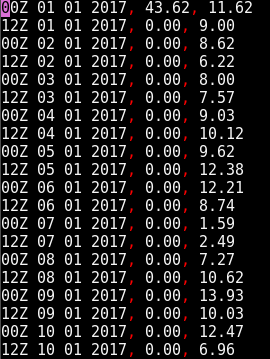
\includegraphics[width=0.3\linewidth]{df2017.png}
\end{figure}

\newpage

El archivo ahora contiene datos para 00Z y 12Z para cada día. Para separar los datos en dos archivos independientes de 00Z y 12Z se pueden utilizar las siguiente instrucciones:
\begin{verbatim}
egrep '00Z' df2017CAPE_PW.csv | cut -d" " -f 2- > df00Z.csv
\end{verbatim}

\begin{verbatim}
egrep '12Z' df2017CAPE_PW.csv | cut -d" " -f 2- > df12Z.csv
\end{verbatim}

Así, tenemos listos los datos para el análisis con Python. En el análisis de Python se utilizaron unas librerías nuevas para gráficar los datos; procedimos a utilizar el ejemplo proporcionado por el profesor para realizar estas gráficas y observar relaciones.

\section{Resultados}

La primera gráfica de caja, que muestra la energía potencial convectiva disponible (CAPE) contra las lecturas por mes, nos dice que en el verano es más propensa la formación de tormentas de rayos debido a que el CAPE representa la capacidad de que se formen estas tormentas. Para ambos tiempos 00Z y 12Z se obtuvieron estos resultados, sin embargo, para el tiempo 00Z la CAPE es mayor a diferencia de al tiempo 12Z.

La segunda gráfica muestra la relación entre el agua precipitable y la CAPE, con la cual se observa que existe una relación lineal entre estos. En ambos tiempos se muestra algo bastante parecido, sin muchas desviaciones.

La tercera gráfica muestra las mismas regresiones lineales, únicamente que en esta gráfica se muestran por cada mes. Las regresiones se muestran bastante parecidas unas con las otras por cada mes.
Para el tiempo 12Z en la tercera gráfica, uno de los meses se encuentra desviado, esto puede ser por error de medición o algo parecido

\section{Conclusión}

Con esta práctica se concluyó que la edición de conjuntos grandes de archivos para la lectura en Python se ven fuertemente facilitadas por comandos en EMACS para seleccionar y reemplazar texto rapidamente.

\newpage

\section{Bibliografía}
\begin{itemize}
\item American Meteorological Society. (13 January 2015). Precipitable water. 03 March 2018, de American Meteorological Society Sitio web: \\http://glossary.ametsoc.org/wiki/Precipitable\_water
\item Instituto meteorológico nacional. (03 November 2015). Elementos importantes para la formación de una tormenta. 03 March 2018, de Instituto meteorológico nacional Sitio web: https://www.imn.ac.cr/documents/10179/16926/1-Elementos+importantes+para+la+formaci\%C3\%B3n+de+una+tormenta.pdf/3c88e1d6-09ca-406e-8323-144a583f7eca
\end{itemize}

\newpage

\title{Apéndice}

\begin{enumerate}
\item ¿Cómo se te hizo esta actividad? ¿Compleja, Difícil, Sencilla? ~\\~\\
Me pareció bastante sencilla, después de aprender exactamente la combinación del teclado para realizar comandos en emacs todo fue muy sencillo.

\item ¿Qué te llamó más la atención?~\\~\\
El manejo rápido de edición de texto para los datos con emacs.

\item ¿Qué parte fue la que menos te interesó hacer?~\\~\\
Utilizar el código del ejemplo sin conocer anteriormente sobre las librerías y algunas gráficas

\item ¿Cómo mejorarías esta actividad? ¿Qué le faltó? ¿Qué sobró?  ~\\~\\
creo que le faltó explicar un poco las gráficas resultantes

\item ¿Hasta este punto, que te parece el uso de Jupyter para programar en Python?  ~\\~\\
Me parece que ha demostrado ser bastante eficiente al gráficar y manejar rapidamente una cantidad grande de datos.

\end{enumerate}

\end{document}
